\chapter{Knowledge Valorisation}
\beginvalorization
The practice of science can be divided into basic and applied science. While basic science is concerned with the investigation and discovery of fundamental principles, applied science is practiced with the aim to solve a specific practical problem, often of a technical nature. The work in this thesis can be understood as basic science. The aim here was to study the principles that describe the relationship between the activity of cortical systems in humans and the contents of visual consciousness.

Valorization is defined as "the process of creating value from knowledge, by making knowledge suitable and/or available for social (and/or economic) use and by making it suitable for translation into competing products, services, processes and new activities" (report of the National Valorisation Committee, Indicators for valorisation, 2011, p. 8). Given the fundamental nature of the research presented in this thesis, the goal was not to create value from knowledge but to create knowledge in the first place. This thesis therefore does not make knowledge directly suitable for social and/or economic use. However, I believe that the work presented here can still be valuable to society in at least two different ways. First, it can bring pleasure to its readers by presenting knowledge about something that is extremely central to our existence - the internal and underlying workings of our brain and mind. Knowing and understanding can be very satisfactory in its own right. Second by organizing, maintaining and creating knowledge and making this knowledge openly available to society, this thesis contributes to the foundation that is absolutely necessary to solving any specific, applied problem. In what follows, these two aspects are elaborated on.

First, humans are innately curious beings, showing an immense drive to explore the environment that surrounds them and often displaying pleasure when discovering new things. Human explorations probably start in mother's womb and if it was not for the drive to explore, none of us would be here today; for the existence of each of us presupposes a long chain of exclusively successful reproductions. These reproductions were successful only because our ancestors followed their drive to forage their environment for appropriate food and mating resources. The human drive to explore, navigate, manipulate and understand our environment is so deeply ingrained that it let us to discover the laws that underlie our immediate and visible surrounding (why does the apple fall from the tree?), discover the laws of particles invisible to the eye and let us to understand the movement of the stars.

A more recent trend in human history is the exploration of the universe inside of our heads rather than of things and processes external to us. The significance of our mental lives for our existence was already pointed out by Rene Descartes. He noted that our internal universe, i.e. our experiences, feelings and thoughts, is the only universe whose existence we can take for granted and, in fact, is the only proof of our very existence. These insights are famously captured by his "Cogito, ergo sum" ("I think, therefore I am"). Given that our mental life is so central to our existence, most humans are curious to learn more about it and its relationship with the brain. By presenting knowledge on this relationship , I think the current thesis has societal value: it affords the pleasure, I hope, of finding things out on a topic that is very central to everyone of us.

Second, given the fundamental nature of this thesis, applied science is required to translate the insights of this thesis into applications. However, it is important to emphasize that basic science, in turn, is a necessary condition for applied science since, in many ways, it relies on the knowledge that is gained in the process of basic science. Imagine we were interested in solving the particular problem of restoring vision in congenitally blind people. These people have been blind from birth - is it in any way possible to give them back vision, even if in a rudimentary form? Tackling such questions is only possible when a rich body of knowledge exists since it requires knowledge in many different aspects: What is a photo-receptor? How does neuronal processing work? How is the light that hits the retina translated into neuronal signals? What are the brain areas involved in visual processing? How are the neuronal signals processed and transformed to give rise to conscious experience of a visual scene? Which neuronal processes render a visual stimulus conscious rather than unconscious? We need to have a basic understanding of all these aspects first before we can address practical questions about restoring vision in the blind. This thesis aims to contribute to such an understanding.

Furthermore, it is important to emphasize that translating fundamental to applied science, is usually not a straightforward process. This is because - by design - most attempts at this translation will fail. Imagine, for example, we were interested in increasing the number of grains that we can harvest from a crop plant - a specific problem of a technical nature. Based on previous fundamental research, we can formulate several hypotheses about potentially effective genetic modifications. Problematically, we do not know which of the modifications will work out in practice, given that it is unclear how the suggested genetic modifications will play out in a complex environment. Furthermore, we do not know, which of the hypothesised modifications, if any, will yield the highest amount of harvest. The hope is that, if we try out ten different modifications, maybe two will work in practice and one of them might increase the harvest by an amount that makes the research efforts worth their while (assuming an exclusively utilitarian perspective on knowledge).

Given these difficulties that are present by design already, it is important not to introduce any additional, unnecessary obstacles to translating knowledge into applications. Such obstacles are difficulties to access the knowledge because it is hidden behind a journal paywall, difficulties to reproduce the process of gaining knowledge because either the custom analysis code or the data are unavailable, or difficulties to understand the knowledge in the first place because the authors did not attempt to use plain language or did not make an effort to visualize what they did in a comprehensible manner. All of these obstacles are still surprisingly common in current scientific practice.

Being aware of these obstacles, we tried to eliminate them whenever possible. This thesis and all of the chapters in it will be made available to the public and free to download for everyone in the world. Two out of three empirical chapters have already been published in journals where articles are openly accessible. Both of these publications were accompanied by the release of code and data that are necessary to perform the described analyses. Furthermore, throughout the thesis, I have attempted to use clear and accessible English and to present comprehensible visualizations of our analysis steps and results. In order raise awareness of the research with a non-expert audience, we also described our research in media outlets such as the in-mind magazine and the Maastricht University news. 

Most of the research presented in this thesis required the development of new software tools. Whenever possible and appropriate, we turned these software tools into open-source packages and made them openly available on GitHub. These packages include the \href{https://github.com/ofgulban/segmentator}{Segmentator package}, \href{https://github.com/MSchnei/pyprf_motion}{the PyPrf Motion package}, \href{https://github.com/MSchnei/pyprf_feature}{the PyPrf Feature package} and \href{https://github.com/MSchnei/hrf_opt}{the Hrf Optimize package}. As illustrated in Figure~\ref{fig:open_source_tool} for the example of the Segmentator package, all of the packages are accompanied by user documentation.

\begin{figure}[!htbp]
\centering
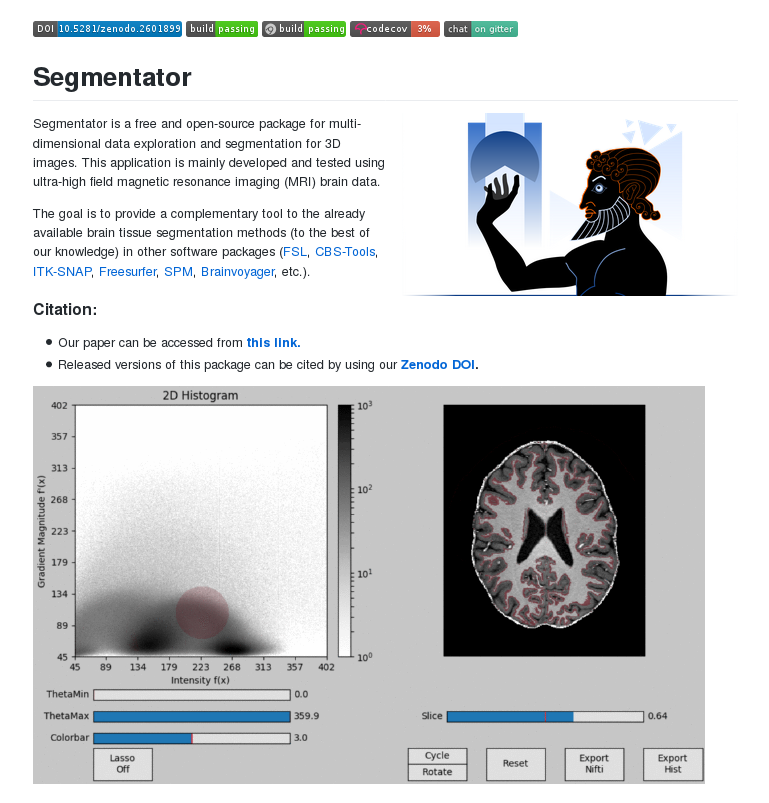
\includegraphics[width=\textwidth]{figures/valorization/segmentator_readme.png}
\caption{Example of open-source software package. As part of this PhD thesis, several software tools were developed that were published on GitHub and accompanied by user instructions}
\label{fig:open_source_tool} 
\end{figure}
\stopsupplement

